% =============================================================================
% PART B - MODULES 10-12: JOB BROWSING, CLIENT JOB MANAGEMENT & BOOKMARKED JOBS
% (UC-10.01 - UC-10.02, UC-11.01 - UC-11.07, UC-12.01 - UC-12.03)
% In Charge: Tran Phat Tai (CE181632)
% =============================================================================

\newpage
\subsection{Modules 10--12: Job Browsing, Client Job Management \& Bookmarked Jobs}

These three modules power the core marketplace discovery and recruitment lifecycle on \textbf{Frevia}. Guests and Freelancers can search, filter, inspect, and bookmark open job postings, while verified Clients can draft, publish, edit, close, reopen, and soft-delete job postings with automated English language validation and non-blocking duplicate-title checks.

% -----------------------------------------------------------------------------
\subsubsection[M10.01 -- View Jobs List (UC-10.01)]{M10.01 -- View Jobs List (Freelancer \& Guest) (UC-10.01)}

\begin{itemize}[leftmargin=1.5em,itemsep=2pt]
  \item \textbf{Screen Name \& Route Path:} Freelancer Find Work -- \texttt{/freelancer/\allowbreak{}find-work/\allowbreak{}most-recent}; Guest Public Jobs -- \texttt{/job}.
  \item \textbf{Target Actor:} Guest, Freelancer, Client (public catalog endpoint).
  \item \Needspace{6\baselineskip}\textbf{Before You Begin:} Open the public Find Work directory or sign in to the Freelancer workspace.
\end{itemize}
\begin{figure}[H]\centering
  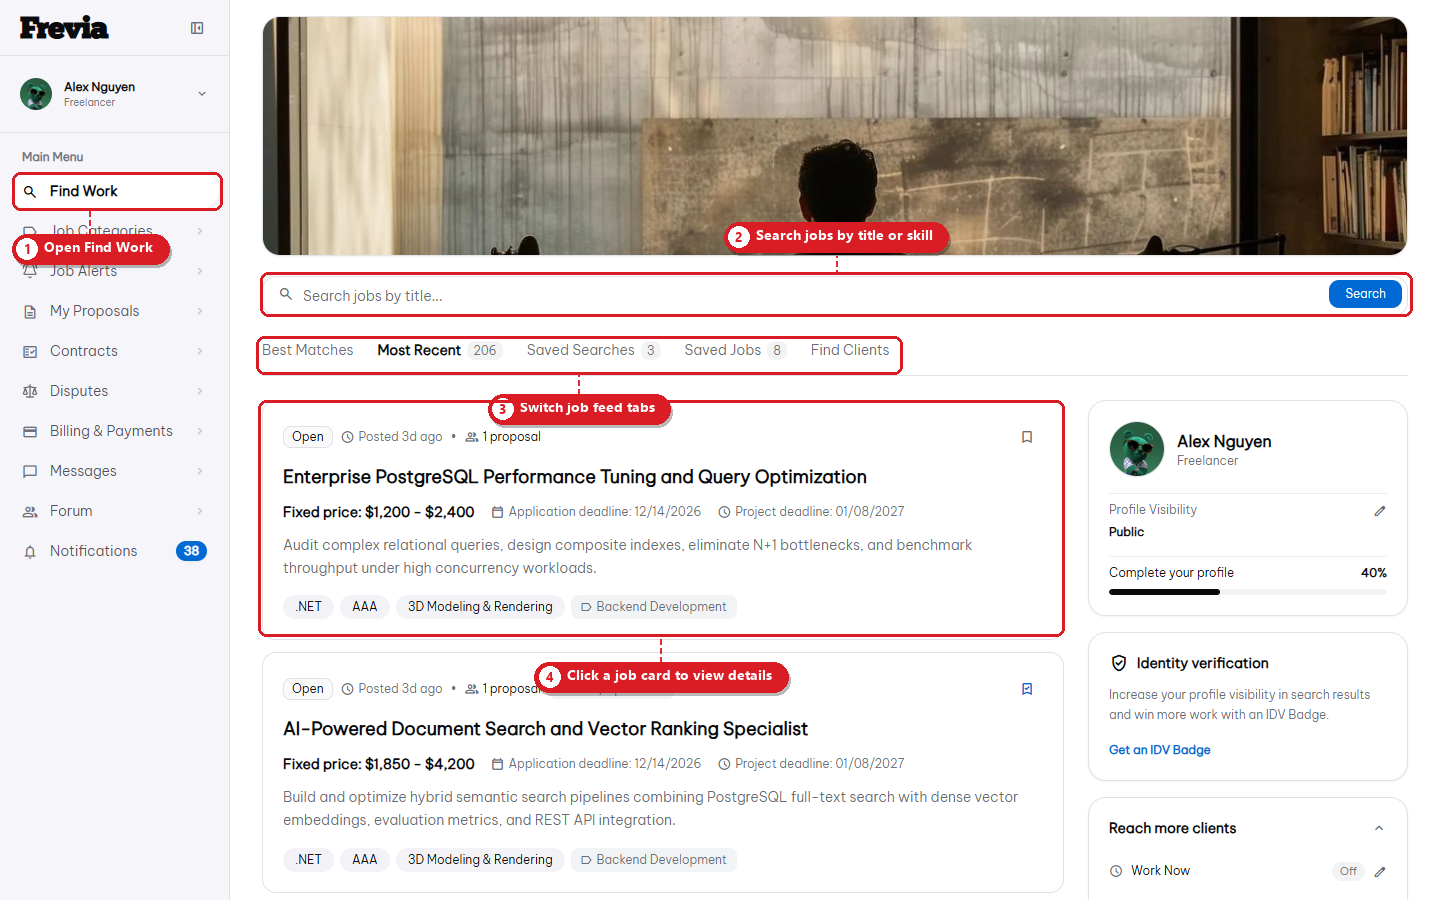
\includegraphics[width=0.90\textwidth]{images/jobs_proposals/m10_01_view_job_list_freelancer_guide.png}
  \caption{Freelancer Find Work feed with search bar, workspace tabs, and open job cards}
  \label{fig:m10_01_view_job_list_freelancer}
\end{figure}
\begin{figure}[H]\centering
  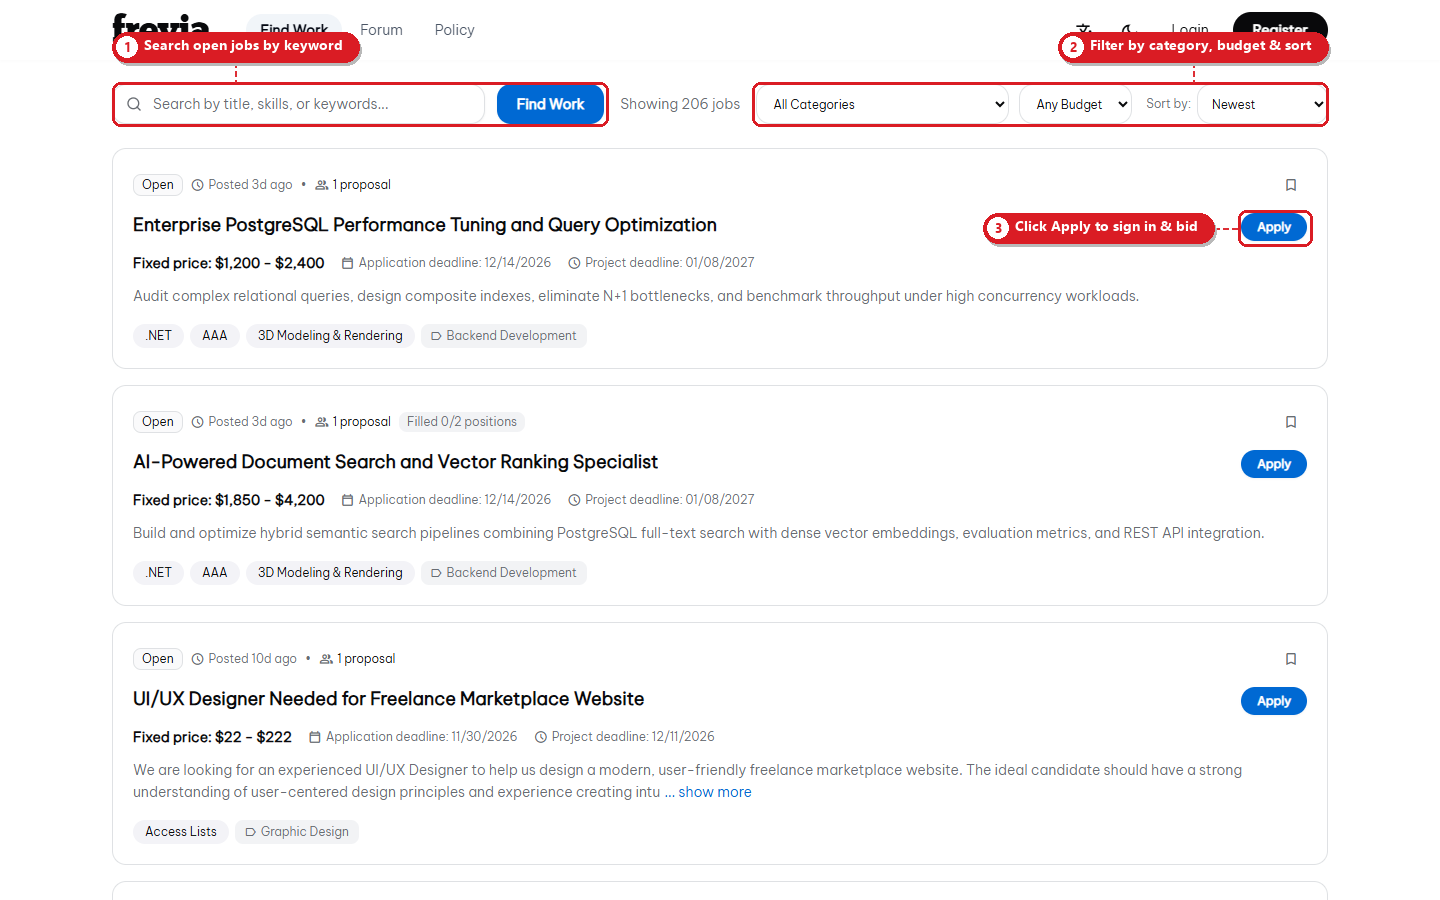
\includegraphics[width=0.90\textwidth]{images/jobs_proposals/m10_01b_view_job_list_guest_guide.png}
  \caption{Public Guest job browsing catalog with keyword search, category, budget, and sort filters}
  \label{fig:m10_01b_view_job_list_guest}
\end{figure}
\Needspace{6\baselineskip}\paragraph{Step-by-Step User Guide:}
\begin{enumerate}[leftmargin=1.8em,itemsep=3pt]
  \item \rbadge{1} \textbf{Open Find Work:} In the Freelancer workspace, click \textbf{Find Work} in the left sidebar (or visit \texttt{/job} as a Guest to search open jobs directly by keyword).
  \item \rbadge{2} \textbf{Search \& Apply Filters:} Enter job title, skill, or keyword terms in the search bar and click \textbf{Search}. On the Guest catalog, combine category, budget range, and sort dropdowns (\textit{Newest}, budget).
  \item \rbadge{3} \textbf{Switch Feed Tabs or Apply:} Switch across \textbf{Best Matches}, \textbf{Most Recent}, \textbf{Saved Searches}, \textbf{Saved Jobs}, and \textbf{Find Clients}. Guests can click \textbf{Apply} on any card to sign in and bid.
  \item \rbadge{4} \textbf{Open a Job Card:} Click any job title card to open its complete specification, required skills, deadlines, and client overview.
\end{enumerate}
\Needspace{6\baselineskip}\paragraph{After You Submit (Result \& Troubleshooting):}
\begin{itemize}[leftmargin=1.5em,itemsep=2pt]
  \item \textbf{What Happens Next:} Only active \texttt{OPEN} non-deleted jobs from non-banned Clients are returned with pagination metadata.
  \item \textbf{Troubleshooting \& Common Messages:} Ensure \textit{Minimum Budget} does not exceed \textit{Maximum Budget}; if no jobs match your active filters, clear filters to view the full catalog.
\end{itemize}

% -----------------------------------------------------------------------------
\newpage
\subsubsection[M10.02 -- View Job Details (UC-10.02)]{M10.02 -- View Job Details (Freelancer \& Client) (UC-10.02)}

\begin{itemize}[leftmargin=1.5em,itemsep=2pt]
  \item \textbf{Screen Name \& Route Path:} Freelancer Job Detail -- \texttt{/freelancer/\allowbreak{}jobs/\allowbreak{}[slug]}; Client Job Detail -- \texttt{/client/\allowbreak{}jobs/\allowbreak{}[jobId]}.
  \item \textbf{Target Actor:} Guest, Freelancer, Client.
  \item \Needspace{6\baselineskip}\textbf{Before You Begin:} Select any job posting from the Find Work catalog, Job Categories directory, or Client My Jobs dashboard.
\end{itemize}
\begin{figure}[H]\centering
  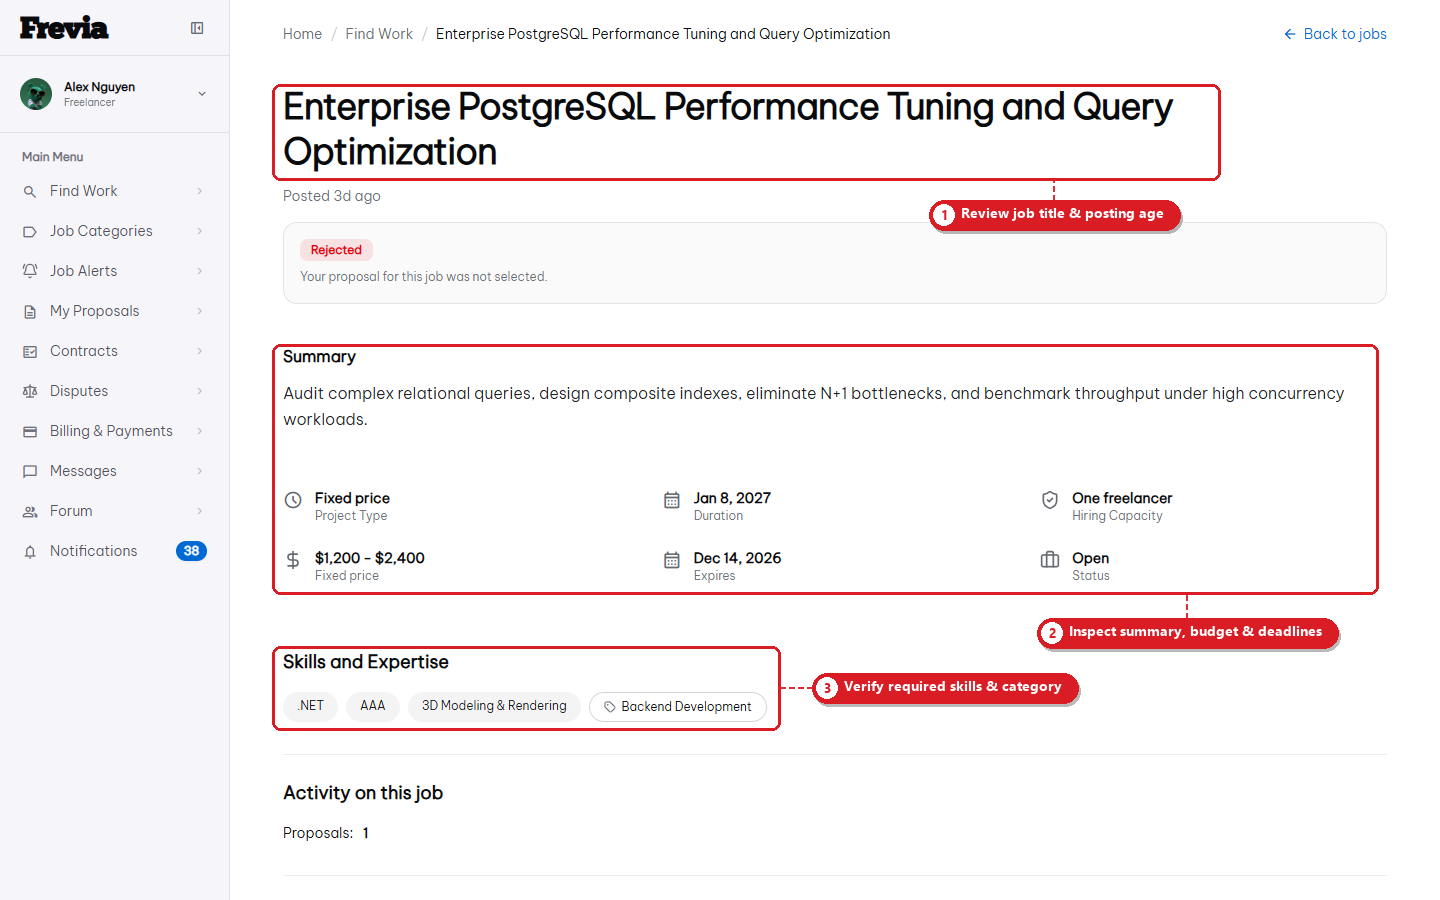
\includegraphics[width=0.90\textwidth]{images/jobs_proposals/m10_02_view_job_detail_freelancer_guide.png}
  \caption{Freelancer Job Detail view showing posting header, summary metrics, and required skills}
  \label{fig:m10_02_view_job_detail_freelancer}
\end{figure}
\begin{figure}[H]\centering
  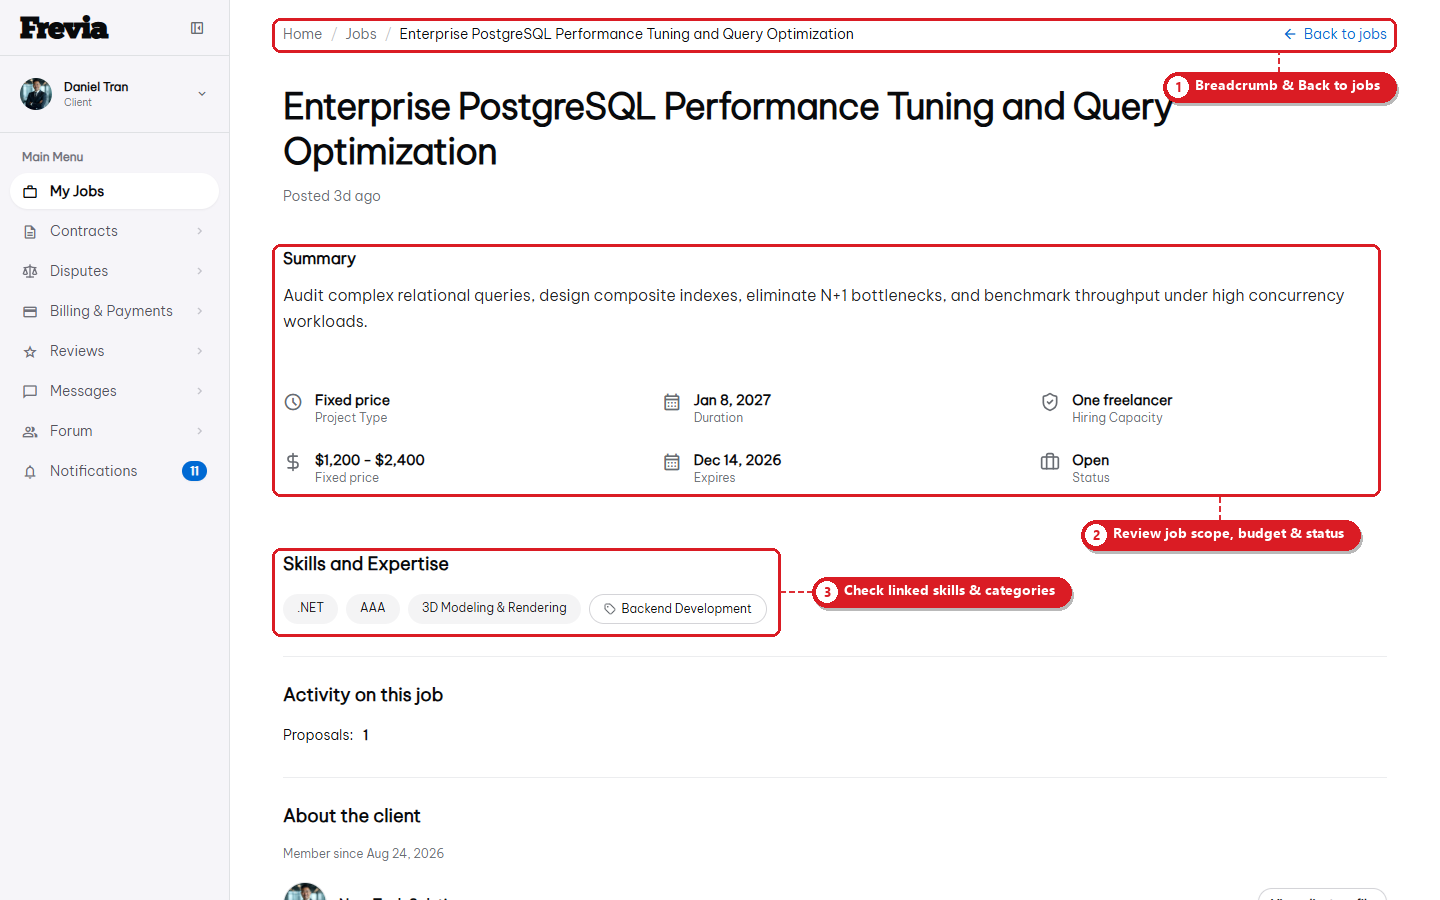
\includegraphics[width=0.90\textwidth]{images/jobs_proposals/m10_02b_view_job_detail_client_guide.png}
  \caption{Client Job Detail view displaying full scope, budget range, status, and linked categories}
  \label{fig:m10_02b_view_job_detail_client}
\end{figure}
\Needspace{6\baselineskip}\paragraph{Step-by-Step User Guide:}
\begin{enumerate}[leftmargin=1.8em,itemsep=3pt]
  \item \rbadge{1} \textbf{Inspect Breadcrumb \& Header:} Review the job title, posting age, and breadcrumb path (or click \textbf{Back to jobs} at the top-right to return to the listing).
  \item \rbadge{2} \textbf{Review Scope, Budget \& Deadlines:} Check the full job summary, fixed-price budget range, hiring capacity (\textit{One freelancer} or \textit{Multiple}), application expiry date, project delivery deadline, and current status.
  \item \rbadge{3} \textbf{Check Required Skills \& Categories:} Verify the linked skill tags, job category badges, proposal count, and client profile details before deciding to bookmark or submit a proposal.
\end{enumerate}
\Needspace{6\baselineskip}\paragraph{After You Submit (Result \& Troubleshooting):}
\begin{itemize}[leftmargin=1.5em,itemsep=2pt]
  \item \textbf{What Happens Next:} Full job attributes, skills, categories, and current proposal status (if already applied) render cleanly.
  \item \textbf{Troubleshooting \& Common Messages:} Accessing an invalid, soft-deleted, or banned client's job slug displays an HTTP 404 \textit{JobNotFound} notice.
\end{itemize}

% -----------------------------------------------------------------------------
\newpage
\subsubsection{M11.01 -- View My Jobs Dashboard (UC-11.01)}

\begin{itemize}[leftmargin=1.5em,itemsep=2pt]
  \item \textbf{Screen Name \& Route Path:} Manage Posted Jobs -- \texttt{/client/\allowbreak{}jobs}.
  \item \textbf{Target Actor:} Client.
  \item \Needspace{6\baselineskip}\textbf{Before You Begin:} Sign in with a Client account and ensure your identity verification (eKYC) is approved to perform recruitment actions.
\end{itemize}
\begin{figure}[H]\centering
  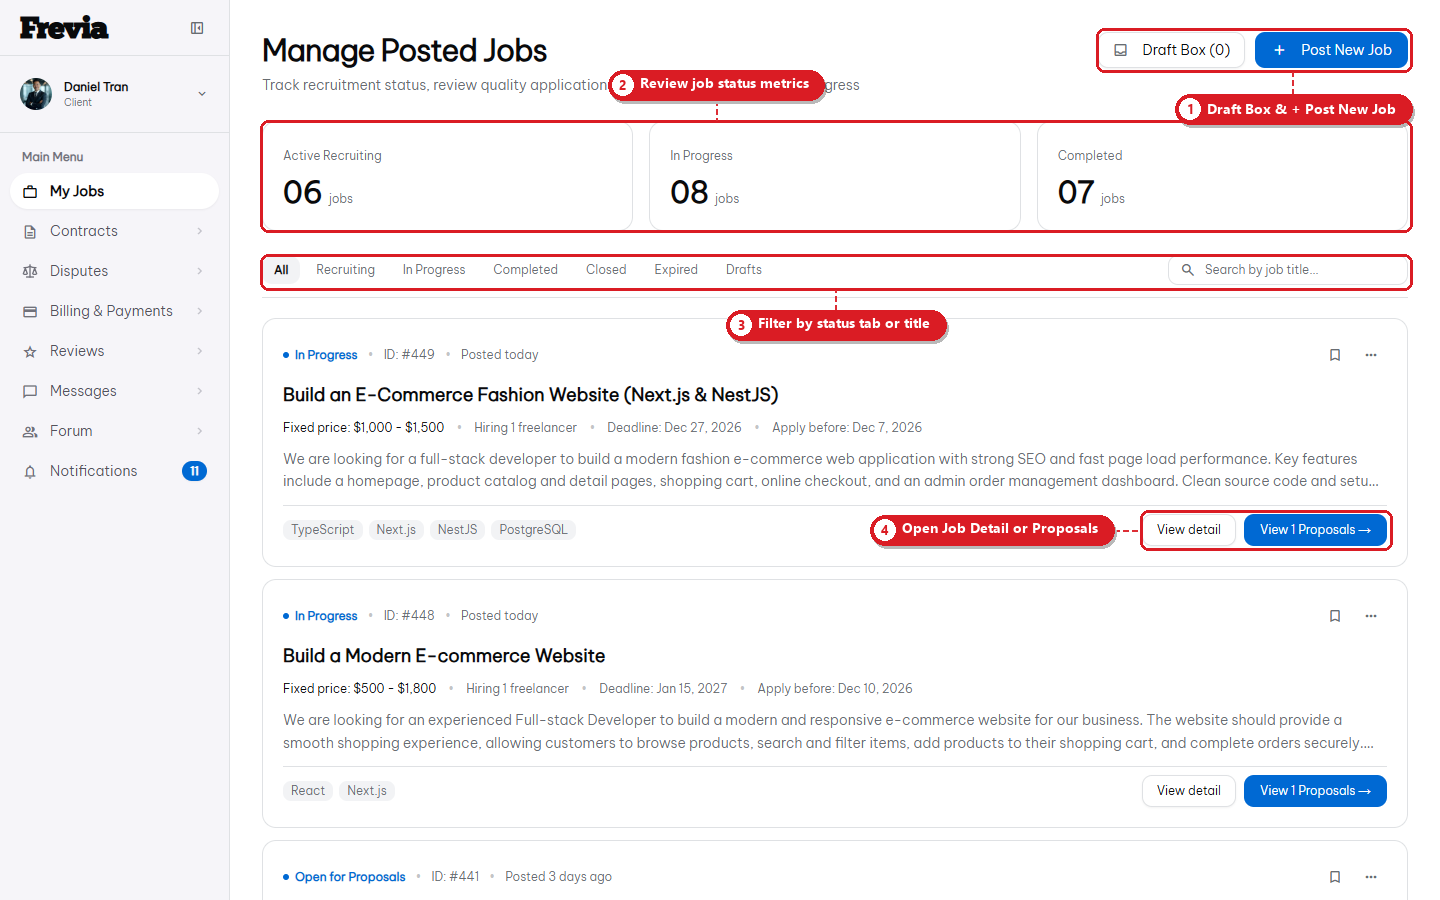
\includegraphics[width=0.90\textwidth]{images/jobs_proposals/m11_01_view_my_jobs_guide.png}
  \caption{Client Manage Posted Jobs dashboard with KPI counters, status filters, and quick actions}
  \label{fig:m11_01_view_my_jobs}
\end{figure}
\Needspace{6\baselineskip}\paragraph{Step-by-Step User Guide:}
\begin{enumerate}[leftmargin=1.8em,itemsep=3pt]
  \item \rbadge{1} \textbf{Open Draft Box or Create New Job:} Click \textbf{Draft Box} to jump directly to unpublished drafts, or click \textbf{+ Post New Job} to open the job creation form.
  \item \rbadge{2} \textbf{Monitor Recruitment Metrics:} Review live counters for \textit{Active Recruiting}, \textit{In Progress}, and \textit{Completed} jobs at the top of the workspace.
  \item \rbadge{3} \textbf{Filter by Status Tab or Search Title:} Switch across \textbf{All}, \textbf{Recruiting}, \textbf{In Progress}, \textbf{Completed}, \textbf{Closed}, \textbf{Expired}, and \textbf{Drafts}, or type keywords in \textit{Search by job title...}.
  \item \rbadge{4} \textbf{Inspect Details or Incoming Proposals:} Click \textbf{View detail} to read the full job specification, or click \textbf{View Proposals} to review freelancer applications.
\end{enumerate}
\Needspace{6\baselineskip}\paragraph{After You Submit (Result \& Troubleshooting):}
\begin{itemize}[leftmargin=1.5em,itemsep=2pt]
  \item \textbf{What Happens Next:} Expired open jobs past their application deadline are automatically closed before the paginated list renders.
  \item \textbf{Troubleshooting \& Common Messages:} Unverified Clients receive an HTTP 403 \textit{IdentityNotVerified} prompt directing them to complete eKYC verification.
\end{itemize}

% -----------------------------------------------------------------------------
\newpage
\subsubsection{M11.02 -- Create Job (UC-11.02)}

\begin{itemize}[leftmargin=1.5em,itemsep=2pt]
  \item \textbf{Screen Name \& Route Path:} Post New Job Form -- \texttt{/client/\allowbreak{}jobs/\allowbreak{}new}.
  \item \textbf{Target Actor:} Client (Identity Verified).
  \item \Needspace{6\baselineskip}\textbf{Before You Begin:} Complete eKYC identity verification (\texttt{APPROVED}) and click \textbf{+ Post New Job} from \texttt{/client/jobs}.
\end{itemize}
\begin{figure}[H]\centering
  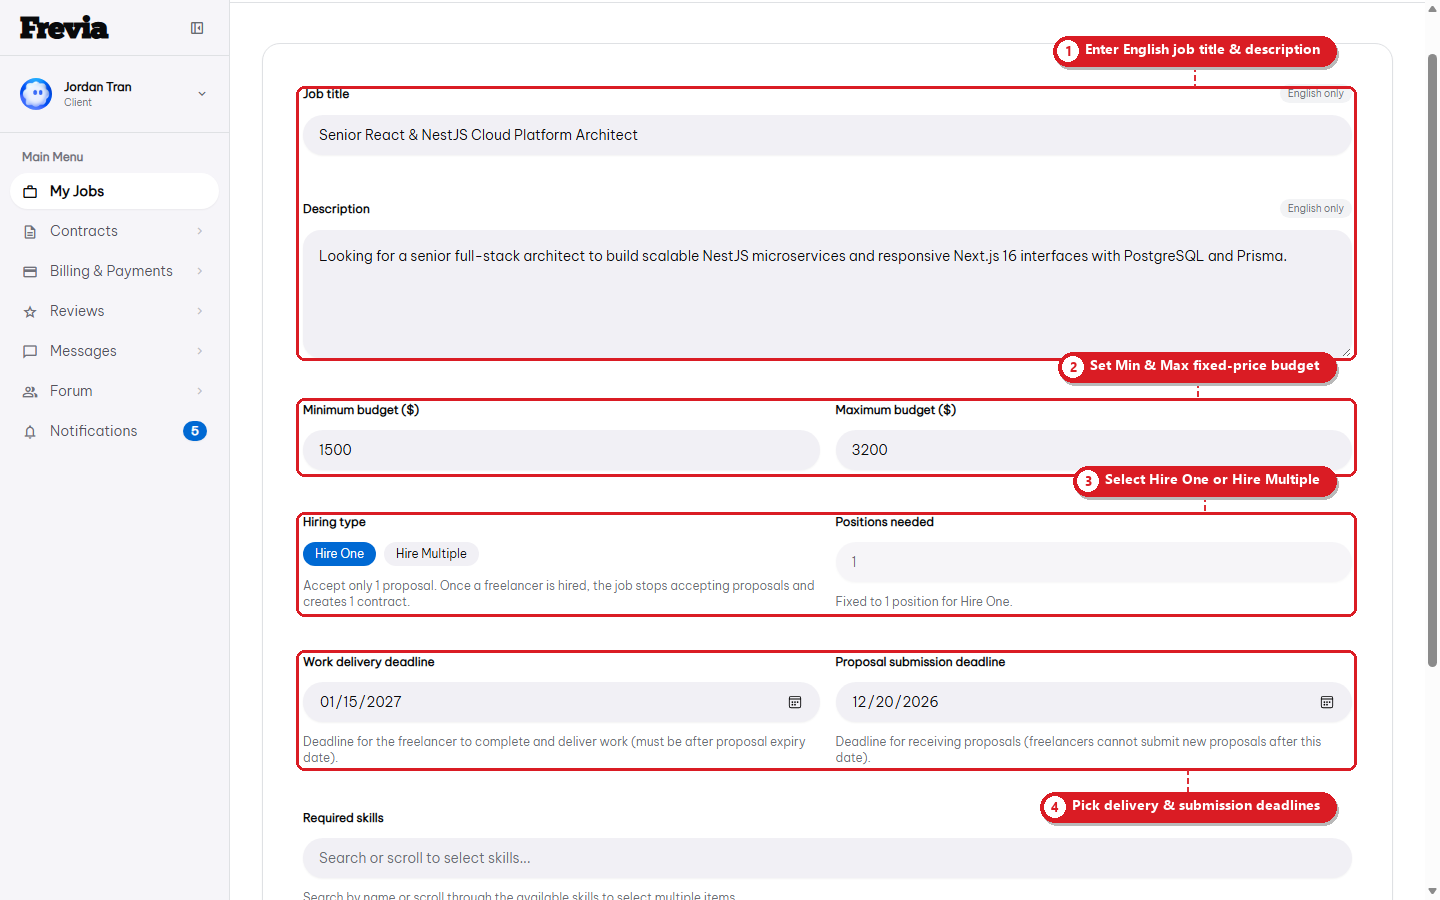
\includegraphics[width=0.90\textwidth]{images/jobs_proposals/m11_02_create_job_guide.png}
  \caption{Post New Job form enforcing English content, fixed budget bounds, hiring mode, and deadlines}
  \label{fig:m11_02_create_job}
\end{figure}
\Needspace{6\baselineskip}\paragraph{Step-by-Step User Guide:}
\begin{enumerate}[leftmargin=1.8em,itemsep=3pt]
  \item \rbadge{1} \textbf{Enter English Job Title \& Description:} Provide a clear English title and detailed technical scope. Both fields are validated automatically by the FastText language detector.
  \item \rbadge{2} \textbf{Set Fixed-Price Budget Range:} Enter positive USD amounts in \textit{Minimum budget (\$)} and \textit{Maximum budget (\$)} such that $\text{Min} \le \text{Max}$.
  \item \rbadge{3} \textbf{Select Hiring Type \& Positions:} Choose \textbf{Hire One} (1 freelancer) or \textbf{Hire Multiple} and specify \textit{Positions needed}.
  \item \rbadge{4} \textbf{Set Deadlines, Skills \& Categories:} Pick a future \textit{Proposal submission deadline} and a later \textit{Work delivery deadline}, select required skills and active job categories, then click \textbf{Save as Draft} or \textbf{Publish Job}.
\end{enumerate}
\Needspace{6\baselineskip}\paragraph{After You Submit (Result \& Troubleshooting):}
\begin{itemize}[leftmargin=1.5em,itemsep=2pt]
  \item \textbf{What Happens Next:} The job, skill links, and category links are persisted inside a single database transaction, and the AI embedding outbox queues the job for recommendation indexing.
  \item \textbf{Troubleshooting \& Common Messages:} Non-English text triggers HTTP 400 \textit{JobMustBeEnglish}; inactive categories return \textit{JobCategoryNotUsable}. If you already own a job with the same title, a non-blocking duplicate-title warning is displayed while still permitting creation.
\end{itemize}

% -----------------------------------------------------------------------------
\newpage
\subsubsection{M11.03 -- Publish Draft Job (UC-11.03)}

\begin{itemize}[leftmargin=1.5em,itemsep=2pt]
  \item \textbf{Screen Name \& Route Path:} Confirm Publishing Job Modal -- \texttt{/client/\allowbreak{}jobs} (\textbf{Drafts} tab).
  \item \textbf{Target Actor:} Client (Job Owner, Identity Verified).
  \item \Needspace{6\baselineskip}\textbf{Before You Begin:} Have at least one saved job in \texttt{DRAFT} status with all required fields (title, description, budget, deadlines, skills, and category) completed.
\end{itemize}
\begin{figure}[H]\centering
  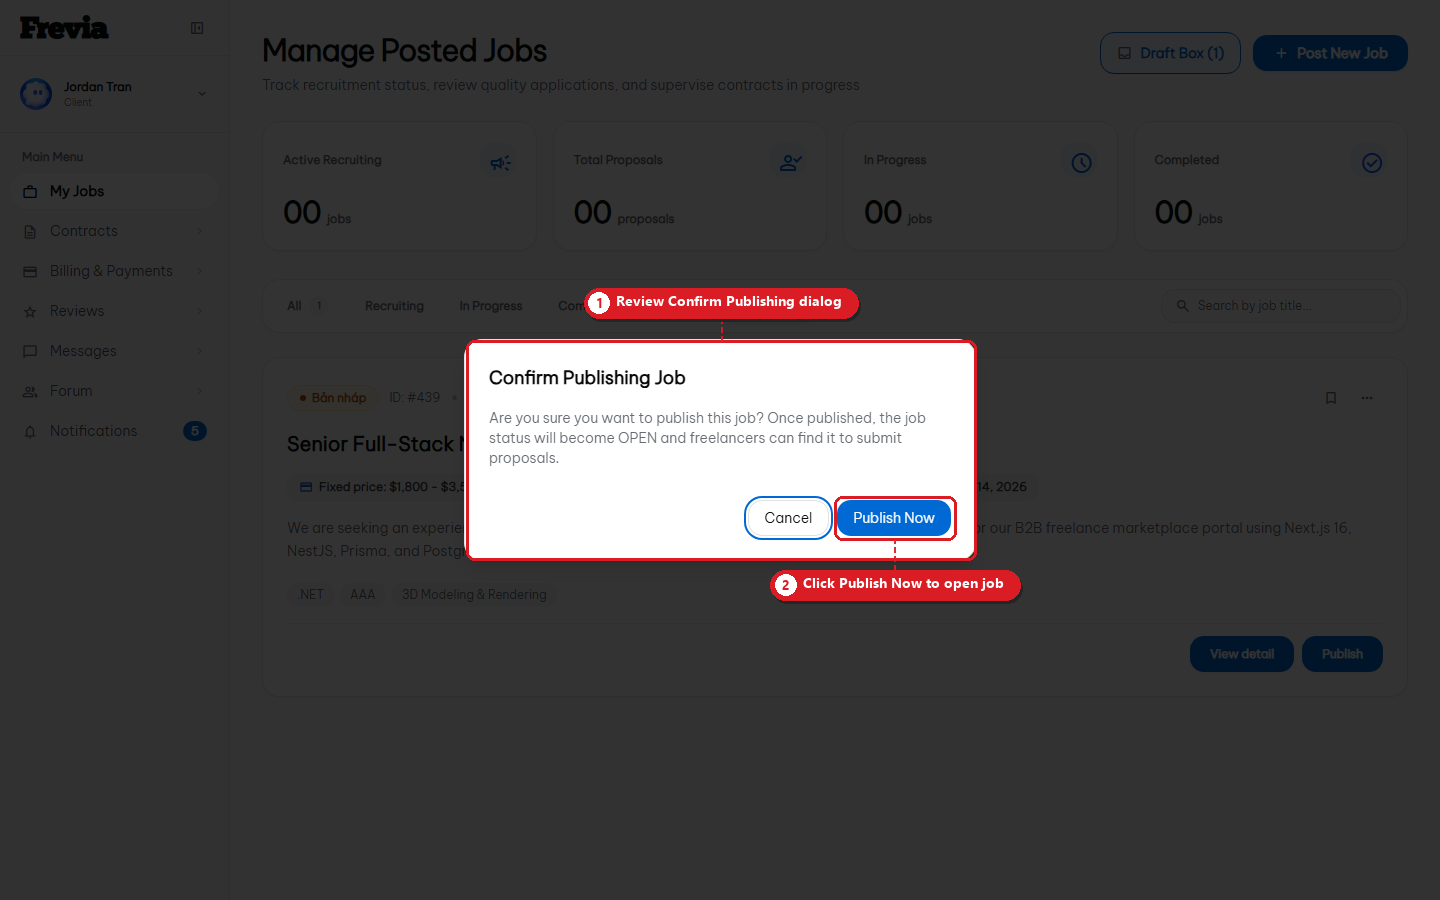
\includegraphics[width=0.90\textwidth]{images/jobs_proposals/m11_03_publish_job_guide.png}
  \caption{Confirm Publishing Job modal transitioning a Draft posting to Open status}
  \label{fig:m11_03_publish_job}
\end{figure}
\Needspace{6\baselineskip}\paragraph{Step-by-Step User Guide:}
\begin{enumerate}[leftmargin=1.8em,itemsep=3pt]
  \item \rbadge{1} \textbf{Open Publish Confirmation:} Navigate to \textbf{My Jobs} $\rightarrow$ \textbf{Drafts}, click \textbf{Publish} on your draft card, and review the confirmation dialog explaining that the job will become publicly visible as \texttt{OPEN}.
  \item \rbadge{2} \textbf{Click Publish Now:} Click the blue \textbf{Publish Now} button (or \textbf{Cancel} to keep the job as a draft).
\end{enumerate}
\Needspace{6\baselineskip}\paragraph{After You Submit (Result \& Troubleshooting):}
\begin{itemize}[leftmargin=1.5em,itemsep=2pt]
  \item \textbf{What Happens Next:} Job status transitions from \texttt{DRAFT} to \texttt{OPEN}, job category cache invalidates, and the posting immediately appears in Freelancer Find Work and AI Best Matches.
  \item \textbf{Troubleshooting \& Common Messages:} Missing required fields or an expired application deadline return HTTP 400 validation errors; edit the draft first before publishing.
\end{itemize}

% -----------------------------------------------------------------------------
\newpage
\subsubsection{M11.04 -- Update Job (UC-11.04)}

\begin{itemize}[leftmargin=1.5em,itemsep=2pt]
  \item \textbf{Screen Name \& Route Path:} Edit Job Slide-Over Sheet -- \texttt{/client/\allowbreak{}jobs}.
  \item \textbf{Target Actor:} Client (Job Owner, Identity Verified).
  \item \Needspace{6\baselineskip}\textbf{Before You Begin:} Open the \texttt{...} action menu on a \texttt{DRAFT}, \texttt{OPEN}, or \texttt{CLOSED} job and select \textbf{Edit}.
\end{itemize}
\begin{figure}[H]\centering
  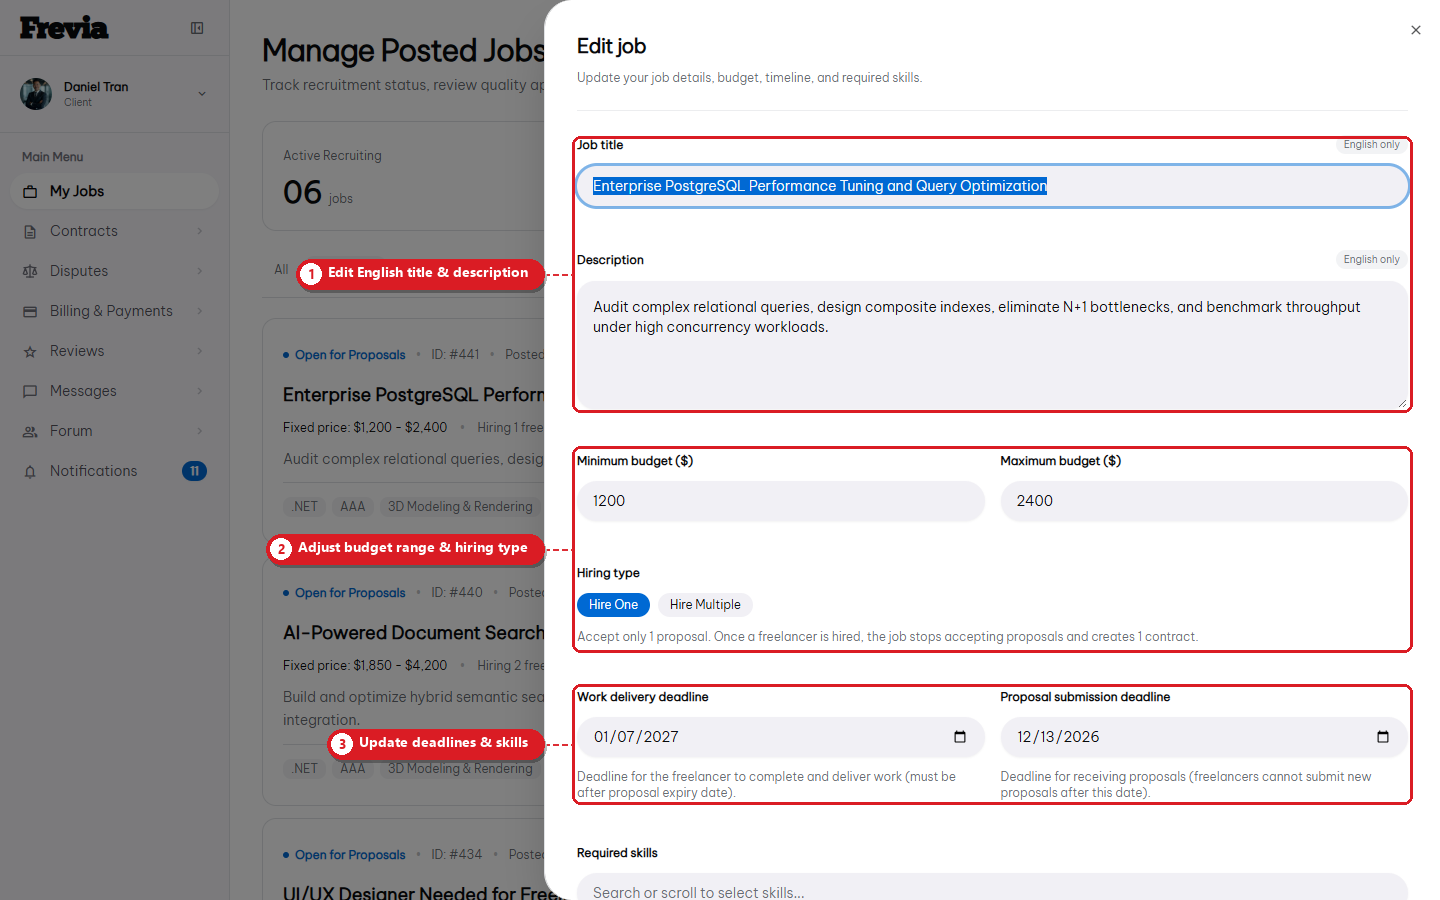
\includegraphics[width=0.90\textwidth]{images/jobs_proposals/m11_04_update_job_guide.png}
  \caption{Edit Job slide-over drawer for updating title, description, budget, hiring type, and schedule}
  \label{fig:m11_04_update_job}
\end{figure}
\Needspace{6\baselineskip}\paragraph{Step-by-Step User Guide:}
\begin{enumerate}[leftmargin=1.8em,itemsep=3pt]
  \item \rbadge{1} \textbf{Modify Title \& Description:} Update the English job title or project description; FastText language validation re-runs automatically on modified text.
  \item \rbadge{2} \textbf{Adjust Budget \& Hiring Type:} Revise \textit{Minimum budget (\$)}, \textit{Maximum budget (\$)}, or switch between \textbf{Hire One} and \textbf{Hire Multiple}.
  \item \rbadge{3} \textbf{Update Deadlines \& Required Skills:} Change the \textit{Work delivery deadline}, \textit{Proposal submission deadline}, skills, or categories, then click \textbf{Save Changes} at the bottom of the drawer.
\end{enumerate}
\Needspace{6\baselineskip}\paragraph{After You Submit (Result \& Troubleshooting):}
\begin{itemize}[leftmargin=1.5em,itemsep=2pt]
  \item \textbf{What Happens Next:} Updated fields, skills, and categories save atomically, and AI embeddings refresh asynchronously.
  \item \textbf{Troubleshooting \& Common Messages:} Jobs already \texttt{IN\_PROGRESS} or \texttt{COMPLETED} cannot be edited; non-English input or invalid date order ($\text{deadline} \le \text{expiryDate}$) is rejected with HTTP 400.
\end{itemize}

% -----------------------------------------------------------------------------
\newpage
\subsubsection{M11.05 -- Delete Job (UC-11.05)}

\begin{itemize}[leftmargin=1.5em,itemsep=2pt]
  \item \textbf{Screen Name \& Route Path:} Delete Job Confirmation Dialog -- \texttt{/client/\allowbreak{}jobs}.
  \item \textbf{Target Actor:} Client (Job Owner, Identity Verified).
  \item \Needspace{6\baselineskip}\textbf{Before You Begin:} Ensure the target job does not have an active contract (\texttt{IN\_PROGRESS}), then click \texttt{...} $\rightarrow$ \textbf{Delete}.
\end{itemize}
\begin{figure}[H]\centering
  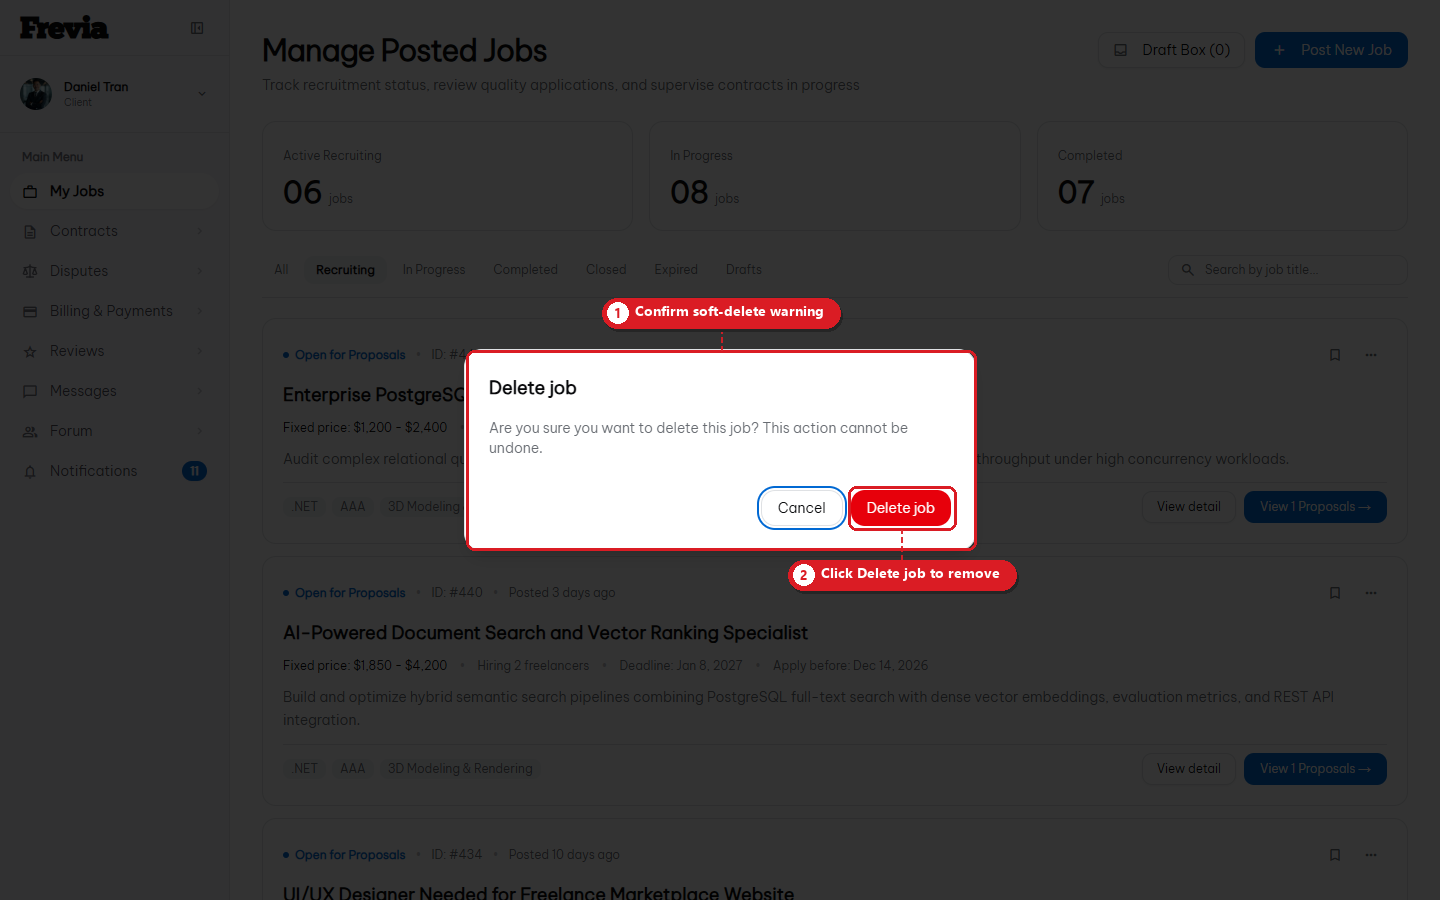
\includegraphics[width=0.90\textwidth]{images/jobs_proposals/m11_05_delete_job_guide.png}
  \caption{Delete Job confirmation dialog prompting permanent soft-deletion of a posting}
  \label{fig:m11_05_delete_job}
\end{figure}
\Needspace{6\baselineskip}\paragraph{Step-by-Step User Guide:}
\begin{enumerate}[leftmargin=1.8em,itemsep=3pt]
  \item \rbadge{1} \textbf{Verify Delete Warning:} Read the confirmation prompt noting that deleting the job removes it from active recruitment listings and cannot be undone by the Client.
  \item \rbadge{2} \textbf{Click Delete Job:} Click the red \textbf{Delete job} button to soft-delete the posting (or \textbf{Cancel} to keep it).
\end{enumerate}
\Needspace{6\baselineskip}\paragraph{After You Submit (Result \& Troubleshooting):}
\begin{itemize}[leftmargin=1.5em,itemsep=2pt]
  \item \textbf{What Happens Next:} The record's \texttt{deletedAt} timestamp is set, removing it from public search and category counts while preserving referential history.
  \item \textbf{Troubleshooting \& Common Messages:} Attempting to delete a job with an ongoing contract returns HTTP 400 \textit{CannotDeleteActiveJob}.
\end{itemize}

% -----------------------------------------------------------------------------
\newpage
\subsubsection{M11.06 -- Close Job (UC-11.06)}

\begin{itemize}[leftmargin=1.5em,itemsep=2pt]
  \item \textbf{Screen Name \& Route Path:} Manage Posted Jobs (\textbf{Recruiting} tab) -- \texttt{/client/\allowbreak{}jobs}.
  \item \textbf{Target Actor:} Client (Job Owner, Identity Verified).
  \item \Needspace{6\baselineskip}\textbf{Before You Begin:} Have an active job in \texttt{OPEN} status on the \textbf{Recruiting} tab.
\end{itemize}
\begin{figure}[H]\centering
  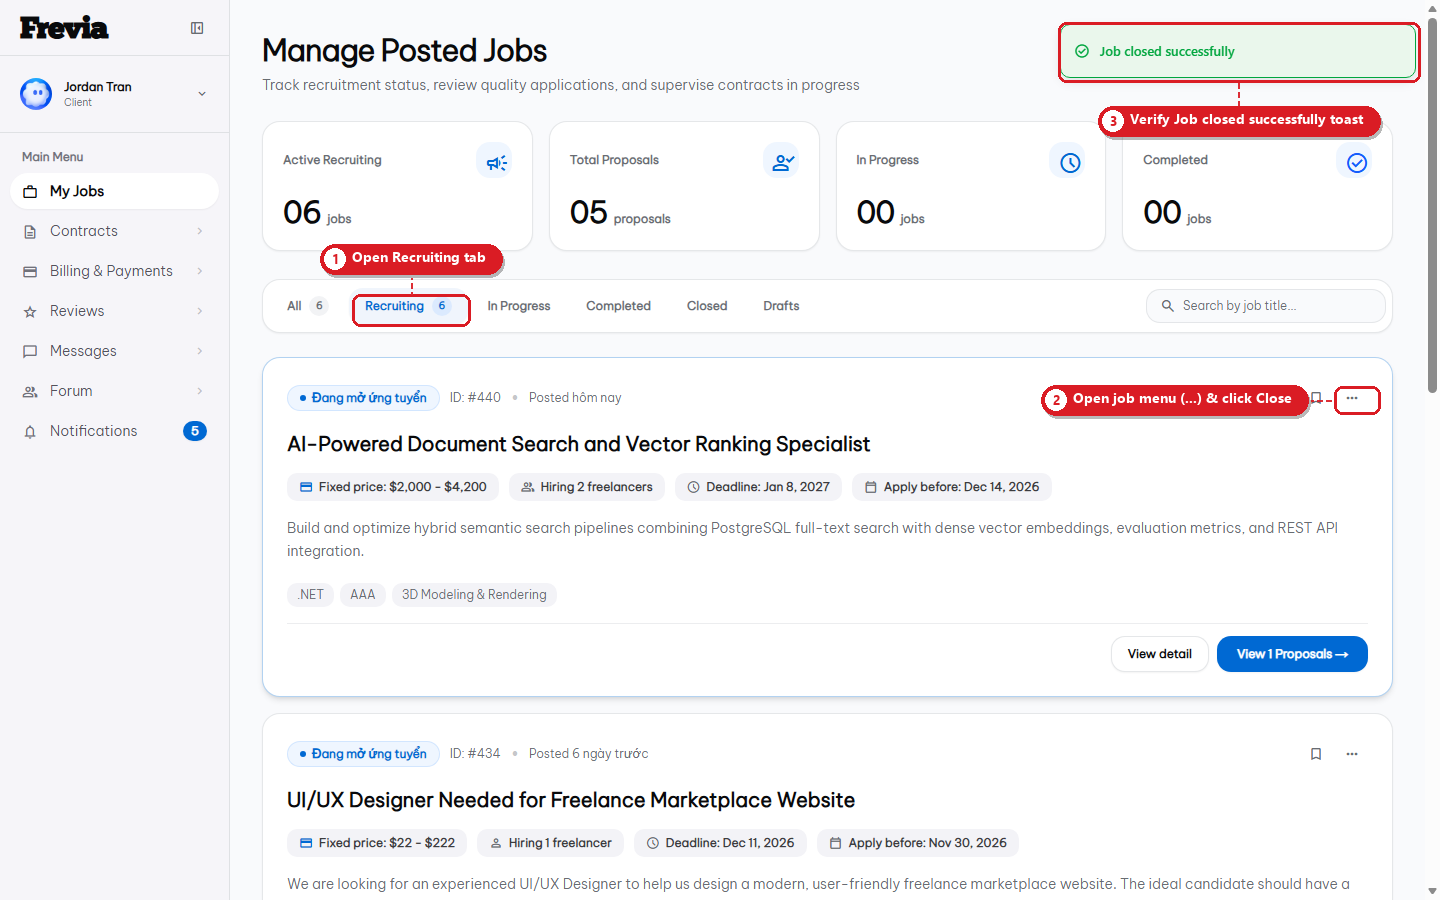
\includegraphics[width=0.90\textwidth]{images/jobs_proposals/m11_06_close_job_guide.png}
  \caption{Closing an active Recruiting job via the job action menu with live confirmation toast}
  \label{fig:m11_06_close_job}
\end{figure}
\Needspace{6\baselineskip}\paragraph{Step-by-Step User Guide:}
\begin{enumerate}[leftmargin=1.8em,itemsep=3pt]
  \item \rbadge{1} \textbf{Open Recruiting Tab:} Select the \textbf{Recruiting} tab to list all currently open job postings.
  \item \rbadge{2} \textbf{Select Close from Job Menu:} Click the three-dot menu (\texttt{...}) at the top-right of the target job card and click \textbf{Close}.
  \item \rbadge{3} \textbf{Confirm Toast Notification:} Verify the green \textit{Job closed successfully} toast in the top-right corner; the job moves to the \textbf{Closed} tab.
\end{enumerate}
\Needspace{6\baselineskip}\paragraph{After You Submit (Result \& Troubleshooting):}
\begin{itemize}[leftmargin=1.5em,itemsep=2pt]
  \item \textbf{What Happens Next:} Status updates to \texttt{CLOSED}, stopping new freelancer proposals immediately and updating category open-job counts.
  \item \textbf{Troubleshooting \& Common Messages:} Only \texttt{OPEN} jobs can be closed; non-open statuses return HTTP 400 \textit{InvalidJobStatusTransition}.
\end{itemize}

% -----------------------------------------------------------------------------
\newpage
\subsubsection{M11.07 -- Reopen Job (UC-11.07)}

\begin{itemize}[leftmargin=1.5em,itemsep=2pt]
  \item \textbf{Screen Name \& Route Path:} Manage Posted Jobs (\textbf{Closed} tab) -- \texttt{/client/\allowbreak{}jobs}.
  \item \textbf{Target Actor:} Client (Job Owner, Identity Verified).
  \item \Needspace{6\baselineskip}\textbf{Before You Begin:} Have a previously closed job in \texttt{CLOSED} status with a valid future application expiry date.
\end{itemize}
\begin{figure}[H]\centering
  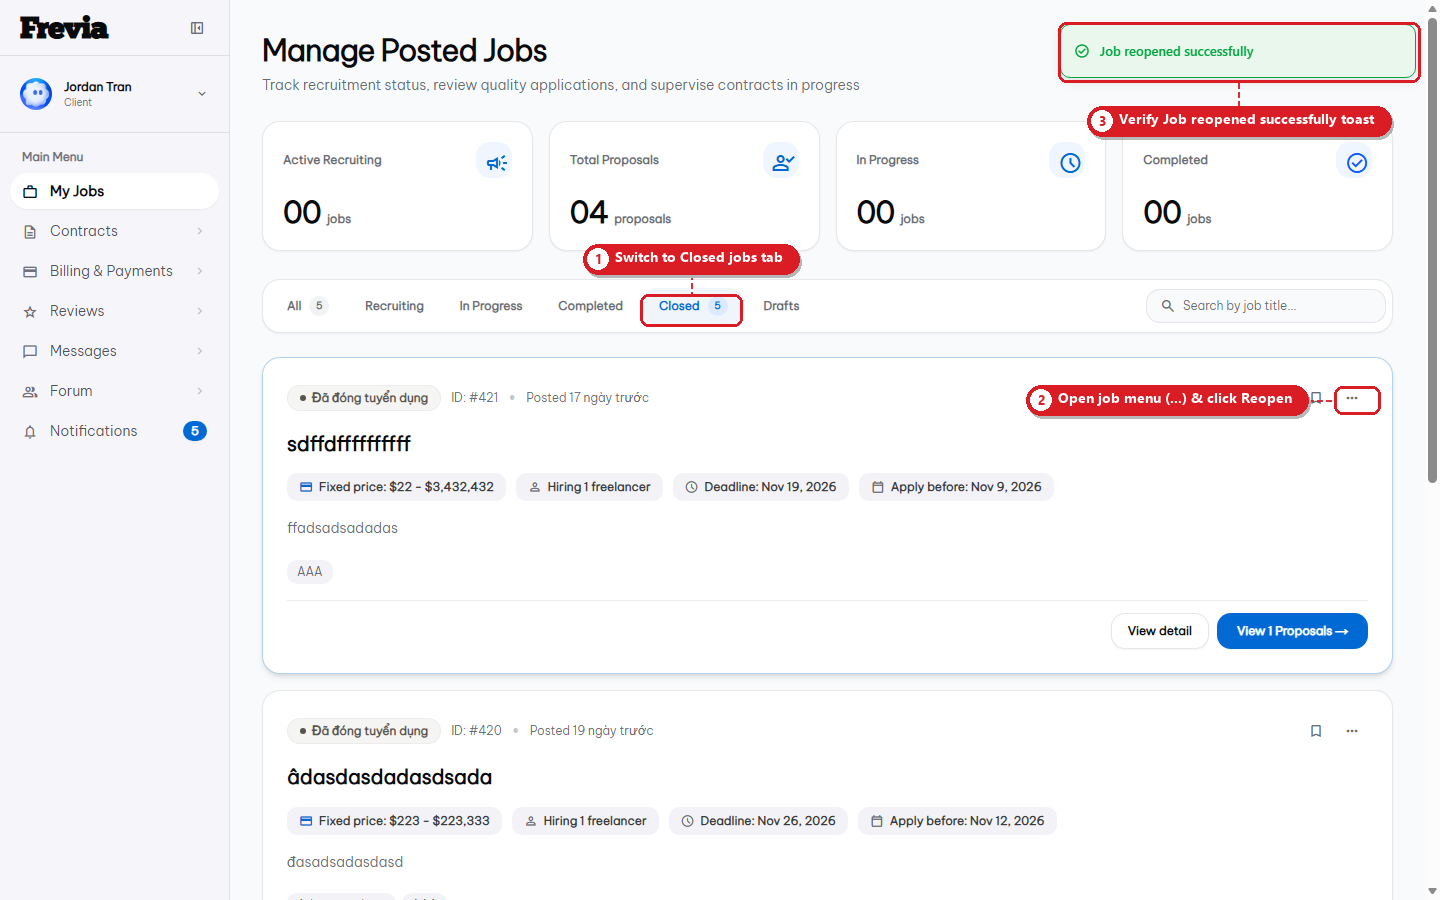
\includegraphics[width=0.90\textwidth]{images/jobs_proposals/m11_07_reopen_job_guide.png}
  \caption{Reopening a Closed job posting from the Closed tab with confirmation toast}
  \label{fig:m11_07_reopen_job}
\end{figure}
\Needspace{6\baselineskip}\paragraph{Step-by-Step User Guide:}
\begin{enumerate}[leftmargin=1.8em,itemsep=3pt]
  \item \rbadge{1} \textbf{Switch to Closed Tab:} Click the \textbf{Closed} status tab in \textbf{Manage Posted Jobs}.
  \item \rbadge{2} \textbf{Select Reopen from Job Menu:} Open the three-dot menu (\texttt{...}) on the closed job card and click \textbf{Reopen}.
  \item \rbadge{3} \textbf{Verify Reopen Confirmation:} Check the green \textit{Job reopened successfully} toast; the job returns to the \textbf{Recruiting} tab as \texttt{OPEN}.
\end{enumerate}
\Needspace{6\baselineskip}\paragraph{After You Submit (Result \& Troubleshooting):}
\begin{itemize}[leftmargin=1.5em,itemsep=2pt]
  \item \textbf{What Happens Next:} Freelancers can once again discover the job and submit proposals, and AI embeddings re-index the posting.
  \item \textbf{Troubleshooting \& Common Messages:} If the job's \textit{Proposal submission deadline} has already passed, edit the job to extend its deadline before reopening.
\end{itemize}

% -----------------------------------------------------------------------------
\newpage
\subsubsection{M12.01 -- View Bookmarked Jobs List (UC-12.01)}

\begin{itemize}[leftmargin=1.5em,itemsep=2pt]
  \item \textbf{Screen Name \& Route Path:} Saved Jobs Tab -- \texttt{/freelancer/\allowbreak{}find-work/\allowbreak{}saved-jobs}.
  \item \textbf{Target Actor:} Freelancer.
  \item \Needspace{6\baselineskip}\textbf{Before You Begin:} Sign in as a Freelancer and save at least one job posting.
\end{itemize}
\begin{figure}[H]\centering
  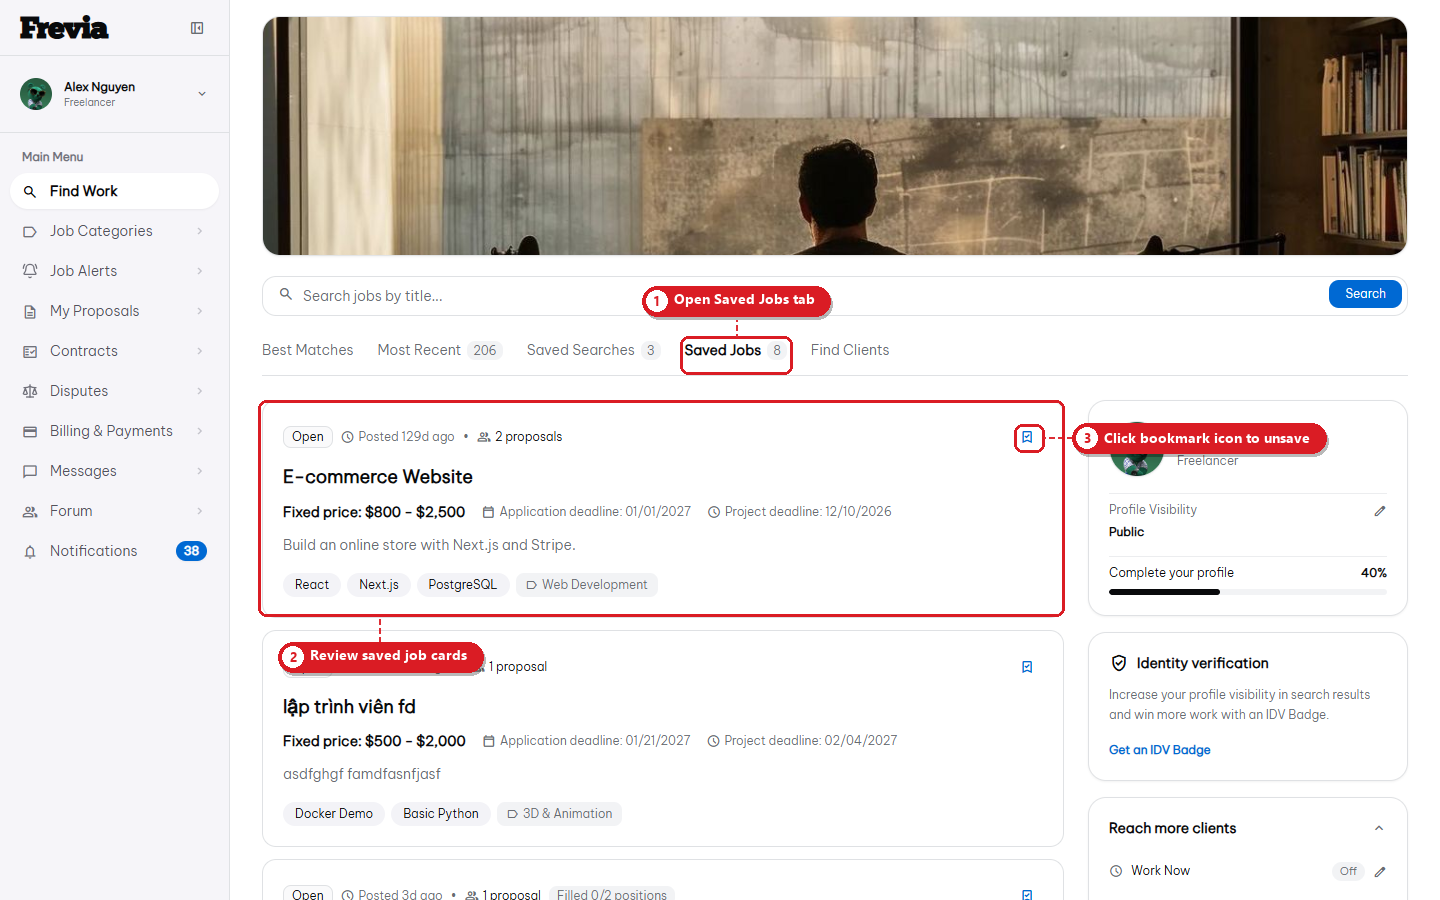
\includegraphics[width=0.90\textwidth]{images/jobs_proposals/m12_01_view_bookmarked_jobs_guide.png}
  \caption{Freelancer Saved Jobs tab displaying bookmarked postings and quick unsave controls}
  \label{fig:m12_01_view_bookmarked_jobs}
\end{figure}
\Needspace{6\baselineskip}\paragraph{Step-by-Step User Guide:}
\begin{enumerate}[leftmargin=1.8em,itemsep=3pt]
  \item \rbadge{1} \textbf{Select Saved Jobs Tab:} From \textbf{Find Work}, click the \textbf{Saved Jobs} tab (showing your current bookmark count badge).
  \item \rbadge{2} \textbf{Browse Saved Job Cards:} Review budgets, application deadlines, skills, and category tags, or click any card title to open the full job detail page.
  \item \rbadge{3} \textbf{Unsave Directly (Optional):} Click the active blue bookmark icon at the top-right of a card to remove it from your saved list.
\end{enumerate}
\Needspace{6\baselineskip}\paragraph{After You Submit (Result \& Troubleshooting):}
\begin{itemize}[leftmargin=1.5em,itemsep=2pt]
  \item \textbf{What Happens Next:} All non-deleted bookmarked jobs load in reverse chronological bookmark order with pagination.
  \item \textbf{Troubleshooting \& Common Messages:} If all bookmarked jobs were removed or deleted by Clients, an empty-state guide invites you back to \textbf{Most Recent}.
\end{itemize}

% -----------------------------------------------------------------------------
\newpage
\subsubsection{M12.02 -- Bookmark Job (UC-12.02)}

\begin{itemize}[leftmargin=1.5em,itemsep=2pt]
  \item \textbf{Screen Name \& Route Path:} Job Detail -- \texttt{/freelancer/\allowbreak{}jobs/\allowbreak{}[slug]} (or job card bookmark icon).
  \item \textbf{Target Actor:} Freelancer.
  \item \Needspace{6\baselineskip}\textbf{Before You Begin:} Sign in as a Freelancer and locate an open job you wish to save for later review.
\end{itemize}
\begin{figure}[H]\centering
  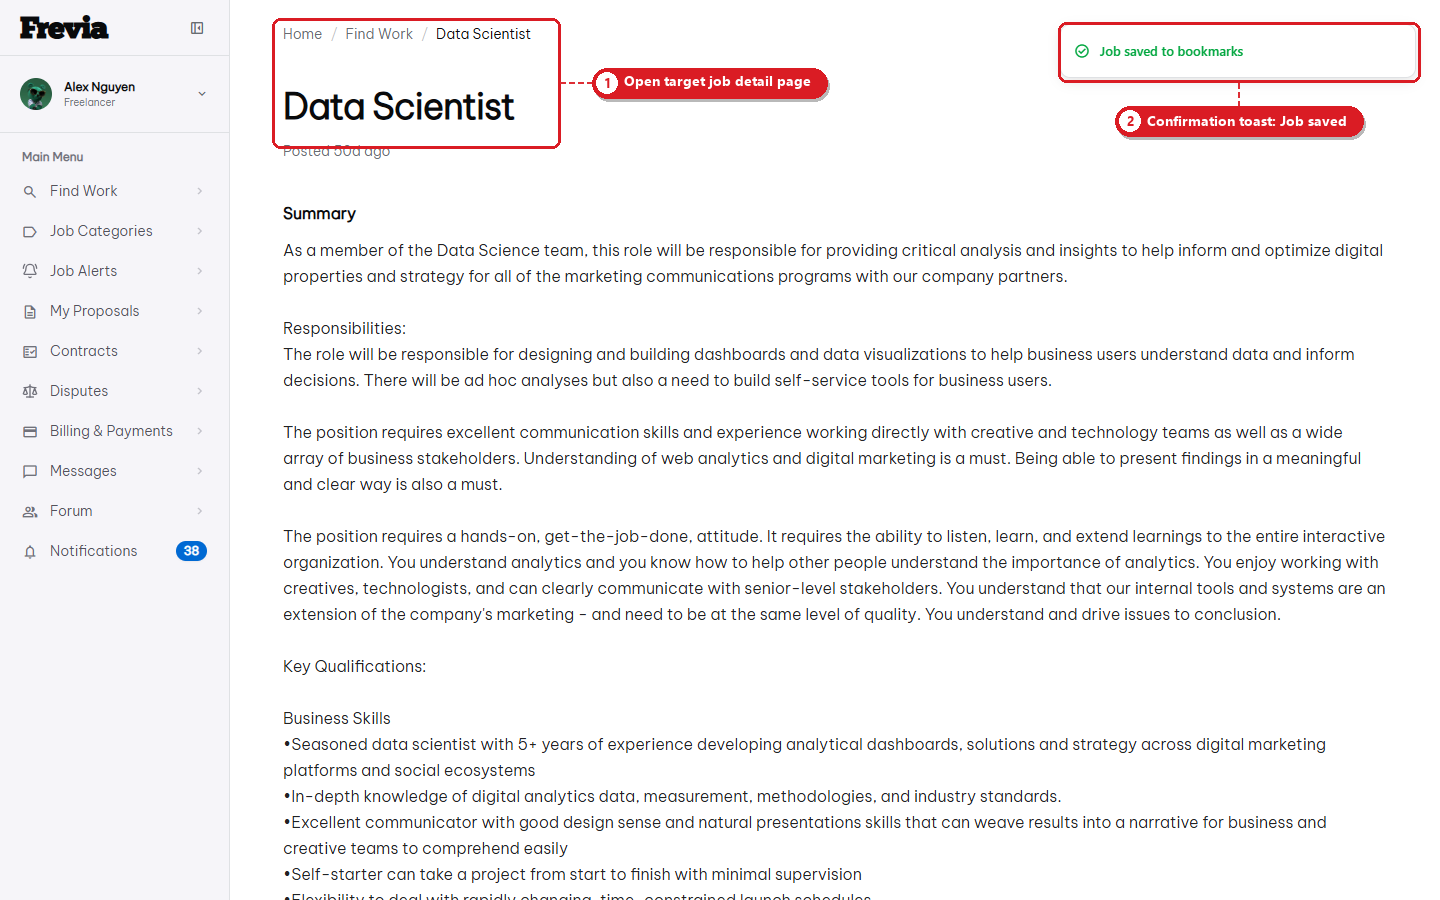
\includegraphics[width=0.90\textwidth]{images/jobs_proposals/m12_02_bookmark_job_guide.png}
  \caption{Job Detail screen displaying the green Job saved to bookmarks confirmation toast}
  \label{fig:m12_02_bookmark_job}
\end{figure}
\Needspace{6\baselineskip}\paragraph{Step-by-Step User Guide:}
\begin{enumerate}[leftmargin=1.8em,itemsep=3pt]
  \item \rbadge{1} \textbf{Open Target Job Detail:} Navigate to the desired open job page and click the \textbf{Save job} bookmark button.
  \item \rbadge{2} \textbf{Verify Bookmark Confirmation Toast:} Confirm the green \textit{Job saved to bookmarks} notification appears in the top-right corner and the button switches to bookmarked state.
\end{enumerate}
\Needspace{6\baselineskip}\paragraph{After You Submit (Result \& Troubleshooting):}
\begin{itemize}[leftmargin=1.5em,itemsep=2pt]
  \item \textbf{What Happens Next:} A \texttt{JobBookmark} record is stored for your account and the \textbf{Saved Jobs} tab counter increments immediately.
  \item \textbf{Troubleshooting \& Common Messages:} Duplicate bookmarks are prevented idempotently; attempting to bookmark a deleted or non-existent job slug returns HTTP 404.
\end{itemize}

% -----------------------------------------------------------------------------
\newpage
\subsubsection{M12.03 -- Remove Bookmark (UC-12.03)}

\begin{itemize}[leftmargin=1.5em,itemsep=2pt]
  \item \textbf{Screen Name \& Route Path:} Remove Saved Job Dialog -- \texttt{/freelancer/\allowbreak{}jobs/\allowbreak{}[slug]} or \texttt{/freelancer/\allowbreak{}find-work/\allowbreak{}saved-jobs}.
  \item \textbf{Target Actor:} Freelancer.
  \item \Needspace{6\baselineskip}\textbf{Before You Begin:} Click the active bookmarked icon on a job you previously saved.
\end{itemize}
\begin{figure}[H]\centering
  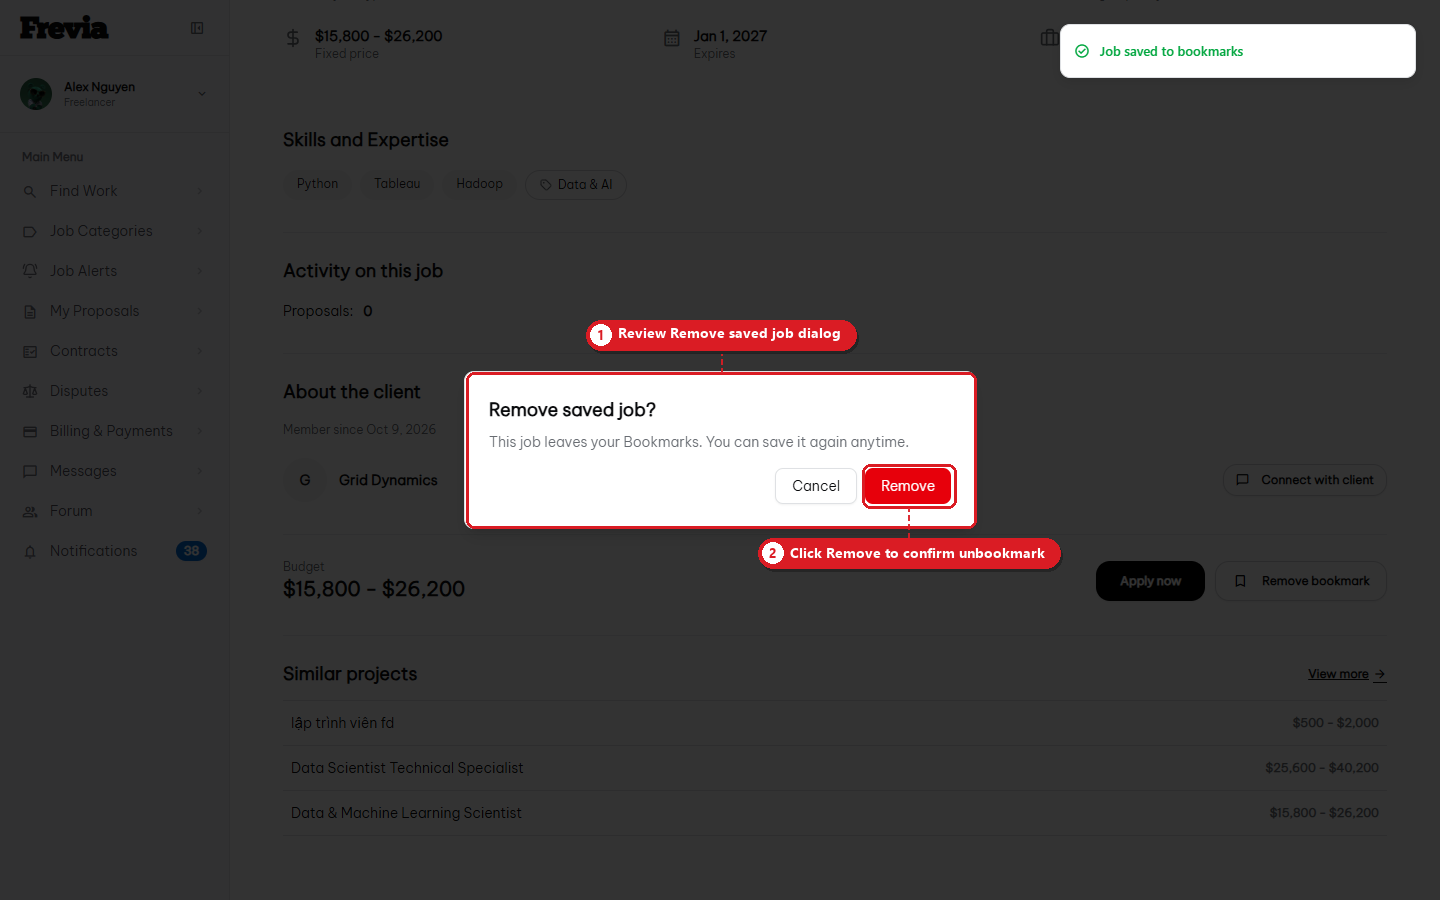
\includegraphics[width=0.90\textwidth]{images/jobs_proposals/m12_03_remove_bookmark_guide.png}
  \caption{Remove saved job confirmation dialog for removing a job from Bookmarks}
  \label{fig:m12_03_remove_bookmark}
\end{figure}
\Needspace{6\baselineskip}\paragraph{Step-by-Step User Guide:}
\begin{enumerate}[leftmargin=1.8em,itemsep=3pt]
  \item \rbadge{1} \textbf{Review Confirmation Dialog:} Inspect the \textbf{Remove saved job?} prompt confirming the job will be removed from your Bookmarks (you can save it again anytime).
  \item \rbadge{2} \textbf{Click Remove:} Click the red \textbf{Remove} button to delete the bookmark (or \textbf{Cancel} to keep it saved).
\end{enumerate}
\Needspace{6\baselineskip}\paragraph{After You Submit (Result \& Troubleshooting):}
\begin{itemize}[leftmargin=1.5em,itemsep=2pt]
  \item \textbf{What Happens Next:} The bookmark is deleted, a \textit{Bookmark removed} toast appears, and the Saved Jobs counter decrements automatically.
  \item \textbf{Troubleshooting \& Common Messages:} If the bookmark was already removed in another tab, the API returns HTTP 404 \textit{BookmarkNotFound} and refreshes the local state.
\end{itemize}
